The Android OS was designed to achieve the best performance when running in mobile devices. This goal brings particular characteristics that developers need to bear in mind when creating Android apps. Some of these characteristics are introduced in this section.

\subsection{Application Not Responding}

Android is built to be highly responsive, which means components may not block on I/O operations on the main thread (also known as the \gls{ui} thread). The system must always be available to respond to user input events. Whenever an application is using the main thread, Android triggers an internal clock that fires when one of the following conditions occurred:

\begin{itemize}
\item No response to an input event within 5 seconds.
\item A BroadcastReceiver hasn't finished executed within 10 seconds.
\end{itemize}

Then, the system launches an \gls{anr} dialog window allowing the user to stop the application's execution, as illustrated in \autoref{fig:anr_dialog}.

\begin{figure}[h]
 \centering
 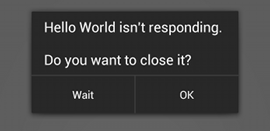
\includegraphics[scale=0.5]{figures/anr_dialog.png}
 \caption{Application Not Responding dialog window}
 \label{fig:anr_dialog}
\end{figure}

To avoid \gls{anr} dialogs, it is recommended to use worker threads in order to execute heavy and long tasks that would block the main thread. The following section introduces the use of worker threads on Android.

\subsection{Worker Threads}

Android consists of four main components that were presented earlier: Activities, Services, Broadcast Receivers and Content Providers. When an application starts executing, Android initiates a new process and, usually, all components run in the same process and thread (main thread). This thread is also called the \gls{ui} thread, because it supports the Android \gls{ui} toolkit components (from the \texttt{android.widget} and \texttt{android.view} packages) that applications interact with. When users provide \gls{ui} events, such as touching a button on the screen, the event is enqueued until the \gls{ui} thread is ready to dispatch it. If some application's component starts a heavy task, by default, it will run on the \gls{ui} thread which may lead to a blocking situation where user input events get stuck on the queue \cite{ProAndroid4:Apress}. This is the typical case where \gls{anr} dialogs are prompted.

Worker threads are used to overcome this problem. In order to take off heavy tasks from the \gls{ui} thread so that it can be ready to handle \gls{ui} events, developers must create other threads to execute such tasks. Note that \gls{ui} events cannot be handled by worker threads, which means that developers may not access the Android \gls{ui} toolkit outside the main thread.